% ============================================================
%  3.1 – Triển khai website và Framework sử dụng  (1 điểm)
%  Trạng thái: ĐÃ HOÀN THIỆN
% ============================================================

\subsection{Kiến trúc tổng thể}

UniJob được triển khai theo kiến trúc \textbf{Serverless SPA} (Single Page Application không
máy chủ riêng), toàn bộ backend được cung cấp bởi Firebase của Google Cloud.

\begin{figure}[H]
\centering
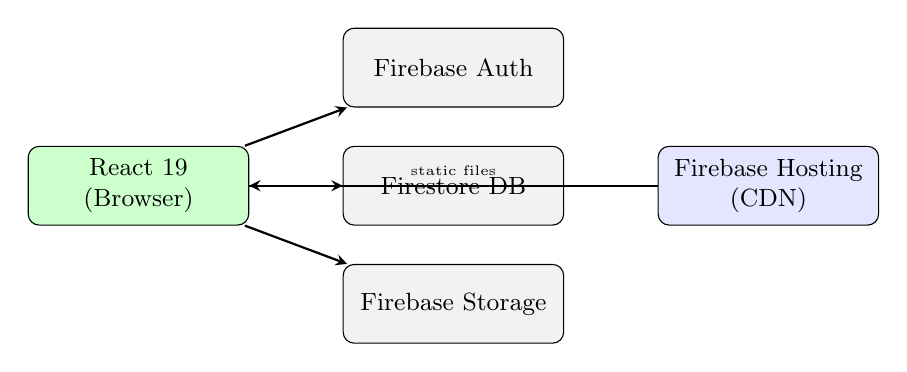
\begin{tikzpicture}[
  box/.style={draw, rounded corners, minimum width=2.8cm, minimum height=1cm,
               fill=gray!10, font=\small, align=center},
  arr/.style={->, thick, >=stealth}
]
  \node[box, fill=green!20] (client) at (0,0) {React 19\\(Browser)};
  \node[box] (auth)  at (4,1.5)  {Firebase Auth};
  \node[box] (db)    at (4,0)    {Firestore DB};
  \node[box] (store) at (4,-1.5) {Firebase Storage};
  \node[box, fill=blue!10] (host) at (8,0) {Firebase Hosting\\(CDN)};

  \draw[arr] (client) -- (auth);
  \draw[arr] (client) -- (db);
  \draw[arr] (client) -- (store);
  \draw[arr] (host)   -- (client) node[midway, above, font=\tiny] {static files};
\end{tikzpicture}
\caption{Kiến trúc triển khai UniJob}
\end{figure}

\subsection{Phân loại tính năng thương mại điện tử}

UniJob không sử dụng framework thương mại điện tử truyền thống (WooCommerce, Shopify...)
mà xây dựng trên nền \textbf{Firebase BaaS} (Backend-as-a-Service) kết hợp với
\textbf{React 19 + Vite}. Bảng dưới đây phân loại tính năng theo tiêu chí e-commerce chuẩn,
phân biệt rõ phần do nền tảng cung cấp sẵn và phần nhóm tự phát triển:

\begin{table}[H]
\centering
\caption{Tính năng e-commerce: Firebase cung cấp vs. nhóm tự phát triển}
\renewcommand{\arraystretch}{1.2}
\begin{tabularx}{\textwidth}{|p{3.2cm}|p{4.6cm}|X|}
\hline
\rowcolor{emeraldrow}
\textbf{\color{emeraldhead}Tiêu chí} &
\textbf{\color{emeraldhead}Firebase cung cấp sẵn} &
\textbf{\color{emeraldhead}Nhóm tự phát triển} \\
\hline
\textbf{Product Management} (Quản lý sản phẩm/task) &
  Firestore CRUD, real-time sync, offline persistence, auto-index &
  Màn hình CreateJob, bộ lọc đa tiêu chí (danh mục, khoa, mức lương, urgent), quản lý trạng thái task (open / assigned / completed) \\
\hline
\textbf{Shopping Cart} (Ứng tuyển / Bookmark) &
  -- &
  Hệ thống ứng tuyển (apply form inline, thư giới thiệu tùy chỉnh), guard chống ứng tuyển trùng, Bookmark danh sách quan tâm lưu trên Firestore \\
\hline
\textbf{Payment Gateway} (Thanh toán) &
  -- &
  Chưa tích hợp trong MVP; thanh toán thỏa thuận trực tiếp giữa hai bên. Lộ trình v2: tích hợp VNPay / MoMo qua Firebase Cloud Functions \\
\hline
\textbf{Mobile Supported} &
  Firebase SDK tương thích mobile browser, PWA-ready &
  Responsive layout Tailwind CSS (\texttt{sm:/md:/lg:}); sidebar bộ lọc collapse thành bottom sheet trên mobile \\
\hline
\textbf{Security} (Bảo mật) &
  Firebase Auth (Google OAuth 2.0), Firestore Security Rules, HTTPS tự động &
  Xác thực domain \texttt{@hcmut.edu.vn}, phân quyền sửa/xóa theo \texttt{uid} người đăng, guard ứng tuyển chính mình \\
\hline
\textbf{Delivery} (Giao nhận / Hoàn thành) &
  -- &
  Cơ chế xác nhận hoàn thành 2 chiều (poster + worker đều confirm), lưu \texttt{jobCompletions}, cập nhật \texttt{workHistory} và mở khóa chức năng đánh giá \\
\hline
\end{tabularx}
\end{table}

\subsection{Frontend -- React 19 + Vite}

\begin{table}[H]
\centering
\caption{Các công nghệ và thư viện frontend chính}
\renewcommand{\arraystretch}{1.2}
\begin{tabularx}{\textwidth}{|p{3.5cm}|p{2.5cm}|X|}
\hline
\textbf{Công nghệ} & \textbf{Phiên bản} & \textbf{Vai trò} \\
\hline
React              & 19.2.0    & UI framework, Concurrent Mode \\
\hline
TypeScript         & 5.9.x     & Type safety, IDE support \\
\hline
Vite               & 8.0.0-beta & Build tool, HMR, tree-shaking \\
\hline
Tailwind CSS       & 4.2.x     & Utility-first CSS, design tokens \\
\hline
React Router DOM   & 7.13.x    & Client-side routing (SPA) \\
\hline
Zustand            & 5.0.x     & Global state (auth, jobs) \\
\hline
TanStack Query     & 5.90.x    & Server state, caching \\
\hline
Framer Motion      & 12.35.x   & Animation, micro-interactions \\
\hline
jsPDF              & 4.2.x     & Tạo file PDF chứng nhận \\
\hline
Lucide React       & 0.577.x   & Icon library \\
\hline
react-hot-toast    & 2.6.x     & Toast notifications \\
\hline
\end{tabularx}
\end{table}

\subsubsection{Cấu trúc thư mục}

\begin{lstlisting}[language={}, caption={Project directory structure}]
unijob-web/
  src/
    components/
      job/        # SuggestedJobs, JobCard
      layout/     # Header, Footer, Layout
    pages/        # Home, JobList, JobDetail, Profile,
                  # CVExport, CreateJob, ...
    services/     # job.service, cv.service,
                  # suggest.service, auth.service, ...
    store/        # authStore (Zustand), jobStore (Zustand)
    types/        # TypeScript interfaces
    lib/          # utils, constants
  firestore.rules
  firebase.json
  .firebaserc
\end{lstlisting}

\subsection{Backend -- Firebase (BaaS)}

\subsubsection{Firebase Authentication}

Sử dụng \textbf{Google OAuth 2.0} là phương thức đăng nhập duy nhất. Người dùng đăng nhập
bằng tài khoản Google, và hệ thống kiểm tra domain email để đảm bảo chỉ email
\texttt{@hcmut.edu.vn} được chấp nhận. Thông tin người dùng (uid, displayName, email,
photoURL) được lưu vào collection \texttt{/users/\{uid\}} sau lần đăng nhập đầu tiên.

\subsubsection{Firestore Database}

Cấu trúc collections chính:

\begin{table}[H]
\centering
\caption{Schema Firestore của UniJob}
\renewcommand{\arraystretch}{1.2}
\begin{tabularx}{\textwidth}{|p{3.2cm}|X|}
\hline
\textbf{Collection} & \textbf{Các trường chính} \\
\hline
\texttt{users}       & uid, displayName, email, faculty, studentId, skills[], ratingScore, avatarUrl \\
\hline
\texttt{jobs}        & title, description, category, faculty, postedBy, status, salary, applicants[], isUrgent, tags[], createdAt \\
\hline
\texttt{applications}& jobId, applicantId, applicantName, message, status, createdAt \\
\hline
\texttt{ratings}     & fromUserId, toUserId, jobId, score (1--5), comment, createdAt \\
\hline
\texttt{jobCompletions} & jobId, workerId, posterConfirmed, workerConfirmed, completedAt \\
\hline
\texttt{workHistory} & userId, jobId, jobTitle, category, completedAt \\
\hline
\end{tabularx}
\end{table}

\subsubsection{Firestore Security Rules}

Bảo mật được đặt ở tầng Firestore với quy tắc rõ ràng:

\begin{lstlisting}[language={}, caption={Firestore Security Rules (excerpt)}]
rules_version = '2';
service cloud.firestore {
  match /databases/{database}/documents {
    function isAuth() {
      return request.auth != null;
    }

    // JOBS: authenticated users can read, only poster can edit/delete
    match /jobs/{jobId} {
      allow read: if isAuth();
      allow create: if isAuth();
      allow update: if isAuth() && (
        resource.data.postedBy == request.auth.uid ||
        request.resource.data.diff(resource.data)
          .affectedKeys().hasOnly(['applicants', 'updatedAt'])
      );
      allow delete: if isAuth()
        && resource.data.postedBy == request.auth.uid;
    }

    // APPLICATIONS: only job poster can change status
    match /applications/{appId} {
      allow create: if isAuth()
        && request.resource.data.applicantId == request.auth.uid;
      allow update: if isAuth() && (
        get(/databases/.../jobs/$(resource.data.jobId))
          .data.postedBy == request.auth.uid
      );
    }
  }
}
\end{lstlisting}

\subsubsection{Firebase Hosting}

Website được deploy lên Firebase Hosting với cấu hình:
\begin{itemize}
  \item \textbf{Project ID:} \texttt{unijob-ad6eb}
  \item \textbf{Build:} \texttt{npm run build} $\rightarrow$ thư mục \texttt{dist/}
  \item \textbf{Deploy:} \texttt{firebase deploy --only hosting}
  \item Tất cả route được rewrite về \texttt{index.html} để React Router hoạt động đúng:
    \texttt{"rewrites": [\{"source": "**", "destination": "/index.html"\}]}
  \item CDN tự động của Firebase phân phối static assets toàn cầu.
\end{itemize}

\subsection{Quy trình CI/CD}

\begin{enumerate}
  \item Developer push code lên nhánh \texttt{feature/xxx} trên GitHub.
  \item Mở Pull Request, review code và kiểm tra build (\texttt{npm run build}).
  \item Merge vào \texttt{main}.
  \item Chạy thủ công: \texttt{npm run build \&\& firebase deploy --only hosting}.
  \item Kiểm tra live URL trên Firebase Hosting.
\end{enumerate}

\subsection{Chi phí vận hành}

\begin{itemize}
  \item \textbf{Firebase Spark Plan (free tier):} Firestore 1 GiB storage, 50k reads/ngày,
    20k writes/ngày -- đủ cho giai đoạn pilot với $<$500 MAU.
  \item \textbf{Firebase Blaze Plan (khi scale):} pay-as-you-go, ước tính
    $\sim$500.000 VNĐ/tháng ở 3.500 MAU.
  \item \textbf{Domain .edu.vn:} $\sim$200.000 VNĐ/năm.
  \item \textbf{Hosting:} bao gồm trong Firebase Spark/Blaze -- không thêm chi phí.
\end{itemize}
